\documentclass[11pt,english]{article}

\usepackage[latin9]{inputenc}
\usepackage[letterpaper]{geometry}
\geometry{verbose,tmargin=1in,bmargin=1in,lmargin=1in,rmargin=1in}
\usepackage{babel}
\usepackage{amsmath}
\usepackage{amssymb}
\usepackage{capt-of}
\usepackage{graphicx}
\usepackage[usenames,dvipsnames]{color}
\usepackage{latexsym}
\usepackage{xspace}
\usepackage{pdflscape}
\usepackage[hyphens]{url}
\usepackage[colorlinks]{hyperref}
\usepackage{enumerate}
\usepackage{ifthen}
\usepackage{float}
\usepackage{array}
\usepackage{tikz}
\usetikzlibrary{shapes}
\usepackage{algorithm2e}

\newcommand{\rthree}{\mathbb{R}^3}
\title{MEAM 620 Advanced Robotics: Assignment 4\\
Due:  Wednesday April 8th}
 \author{Gabrielle Merritt}
 
\date{}

\begin{document}
\maketitle
In all the problems below, you might find a close problem in the literature. We recommend that you do not look into the literature. If you still commit the ``crime'' and find a solution in the literature, please cite the exact source you followed to write the solution. 
No citation of the source will result in ZERO points. The problems are stated in such a way that we can see whether you followed a 3rd party solution (in most cases we ask for a specific unknown to be computed).


\begin{enumerate}

\item [40pts]
 A circle has known radius $\rho$ and can be assumed to be in the $Z=0$ plane centered at $(0,0,0)$ origin of a world coordinate system. A quadrotor observes the circle as an ellipse in the image plane (this is not always the case but we assume that the quadrotor is sufficiently far). Compute the altitude ($Z$) of the quadrotor in the world coordinate system as well as its distance to the circle center. 
Which other degree(s) of freedom of the quadrotor can be computed?

\paragraph{Solution for altitude:}

we can rewrite the equation of a circle and the equation for an ellipse in matrix form as 

Circle: 
\begin{equation}
C = \begin{pmatrix}
1 & 0 & 0 \\ 
0&1&0 \\ 
0&0& -\rho^2 
\end{pmatrix}
\end{equation}

Ellipse: 
$$
L = \begin{pmatrix}
a^2& 0 & 0 \\ 
0&b^2&0 \\ 
0&0& -1 
\end{pmatrix}
$$
$$
E = R L R^T
$$

We can rewrite these equations as 
\begin{equation}
x_c^T E x_c = 0 
\end{equation}
\begin{equation}
x_w^T C x_w = 0
\end{equation}


Our normal Transformation equation can be written as 
Where H is our homography transformation
 \begin{equation}
 \lambda x_c = H x_w 
 \end{equation}
 
 We can also rewrite H as 
 $$ H = \begin{bmatrix}
 r_1& r_2 & t 
 \end{bmatrix}
 $$ 
 and the determinate of H can be written as 
 \begin{equation}
 \det{H} = t\cdot (r_1 \times r_2) = t \cdot r_3 
 \end{equation}
 
 If we look at the problem graphically we can specify that  $ r_1$ points from the center of the circle on the same plane, and that $r_3$ aligns with altitude of the camera 
 \begin{figure}[h!]
  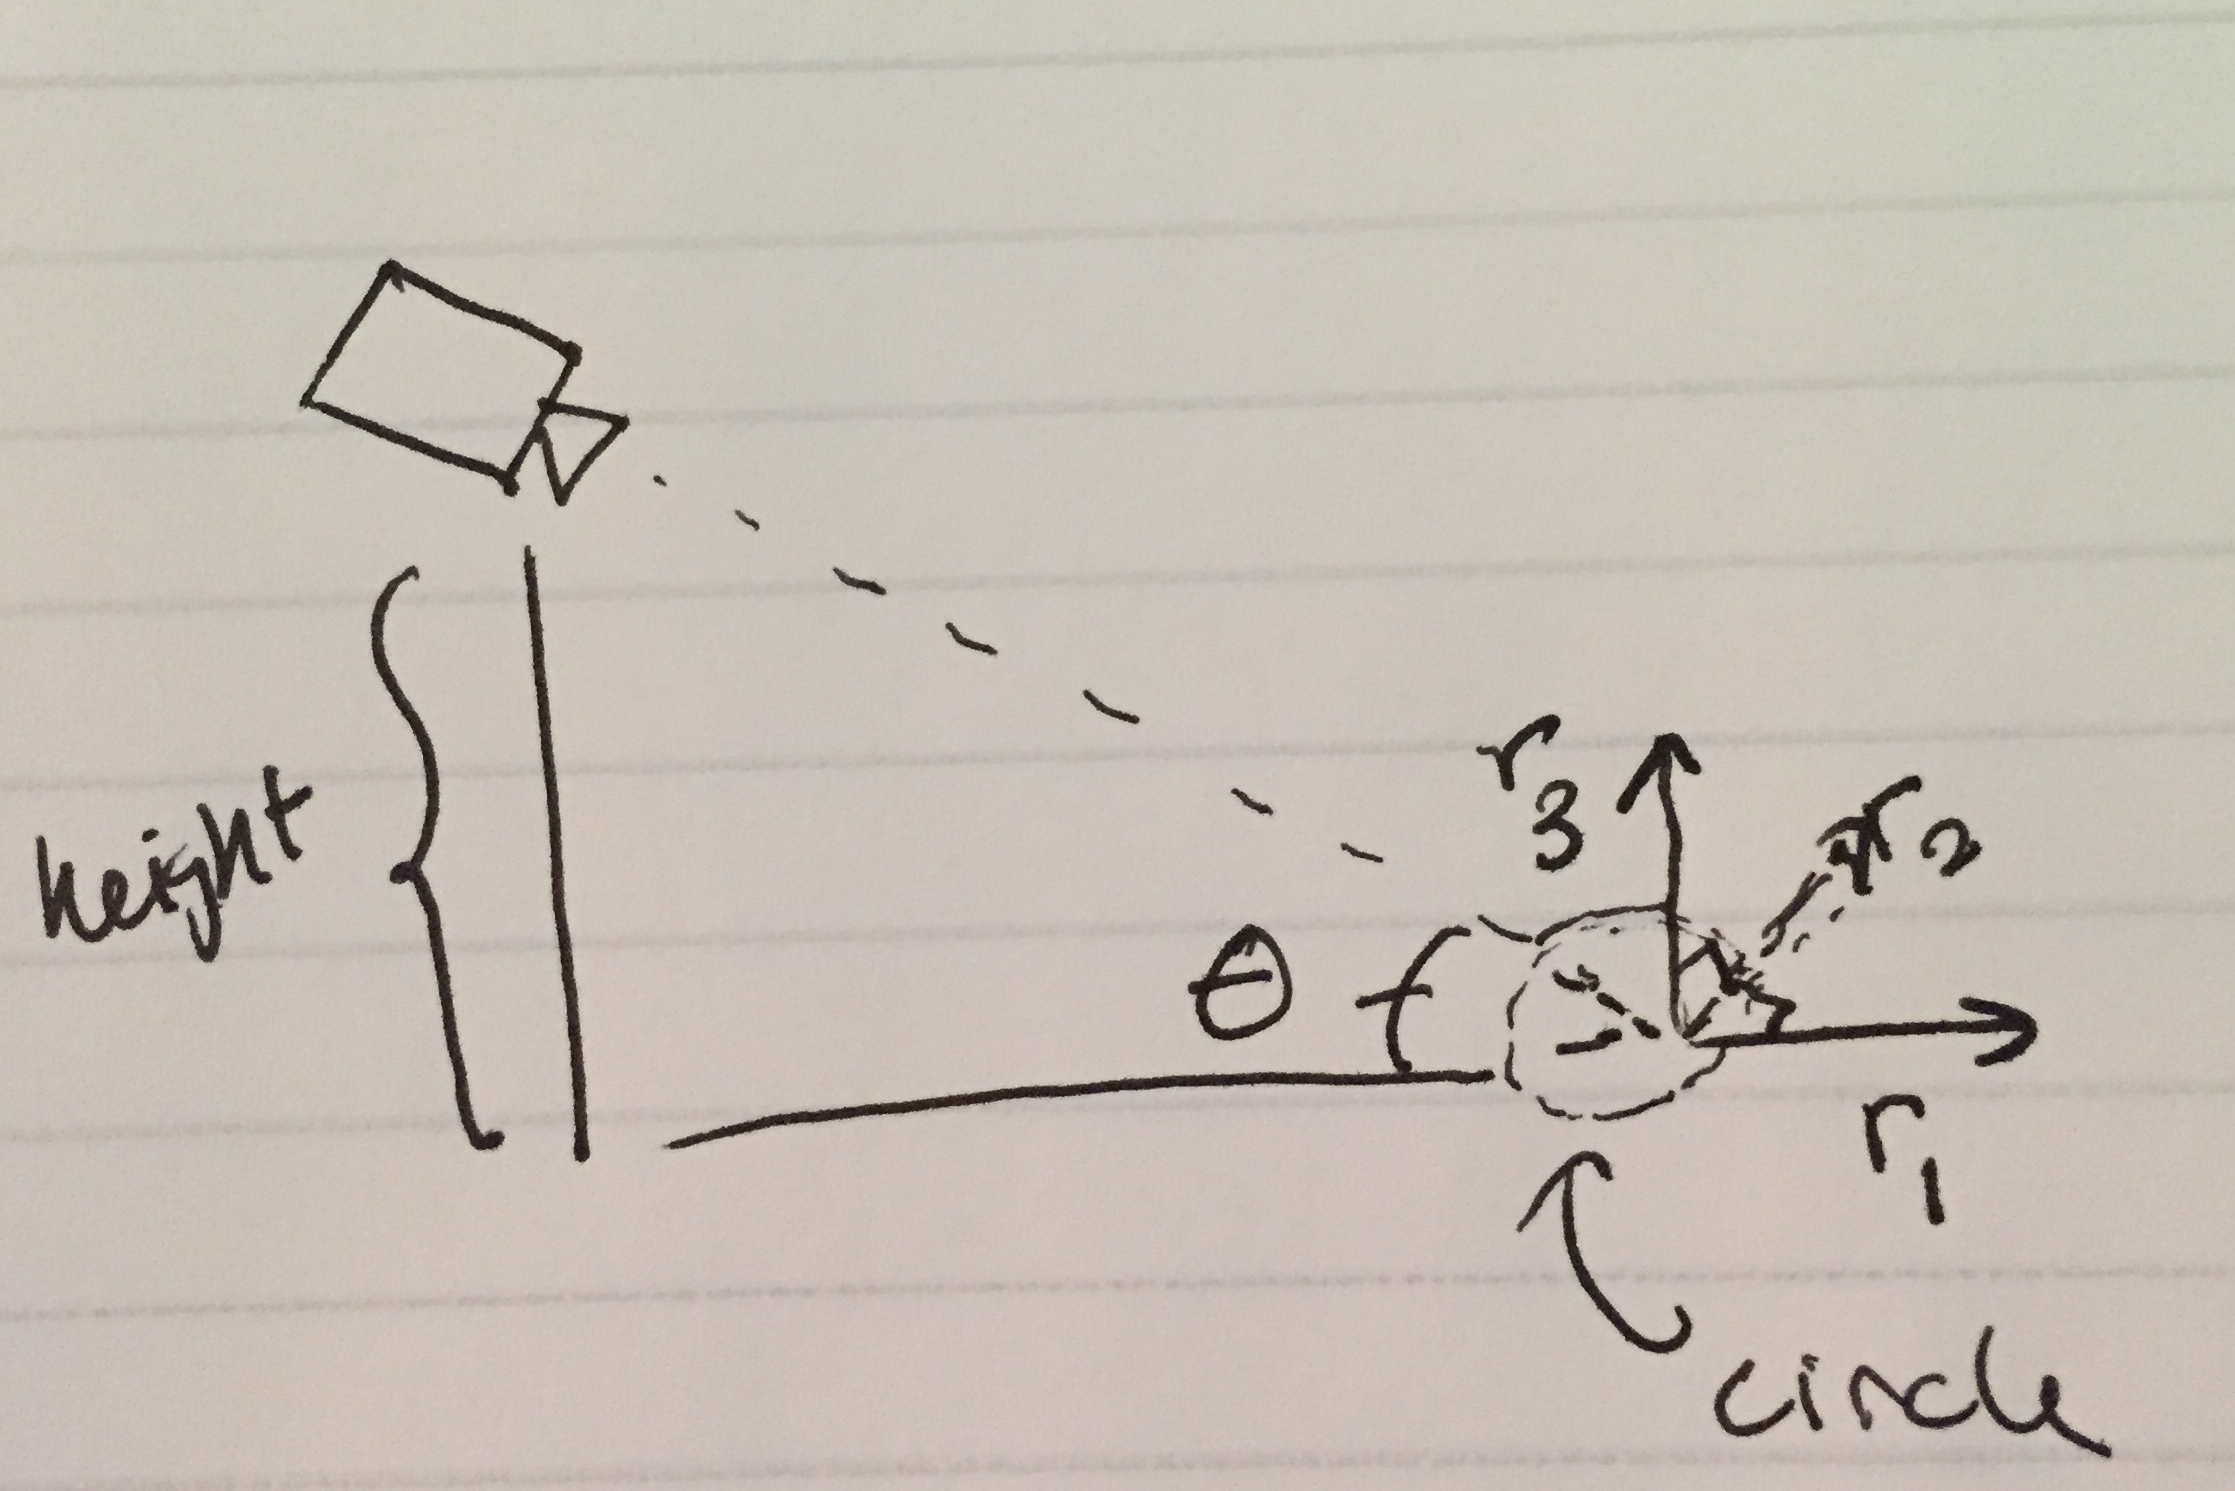
\includegraphics[width = \linewidth]{camera}
\caption{camera looking at circle}
 \end{figure}
 
 By substituting $ H x_w$ for $x_c$ in equation 2. We have:  
 \begin{equation}
 x_w^T H^T E H x_w = 0 
 \end{equation} 
 In this form we can see that  
 $$  x_w^T H^T E H x_w = 0   = x_w^T C x_w = 0 $$ 
 $$ H^T E H = C $$ 
We can take the determinants of each of the elements in the equation above to find a value for $t \cdot r_3  $ 
$$
\det H^2 \det E = \det C = - \rho^2   
$$
\begin{equation}
\det H = \sqrt{\frac{-\rho^2 }{ (a^2b^2)}} = t \cdot r_3 
\end{equation} 

\paragraph{Solution for distance from center of circle}

 In order to find the distance from the circle center and the altitude of the quadrotor we have    to find the skew and rotation of the ellipse in the camera frame. 
 We can do this by moving around equations 2,3,4. and re writing $H^-T x_c$ for $x_w$ 
 we get : 
 \begin{equation}
 x_c^T H^{-T} C H^{-1} x_c = 0
 \end{equation}
 Since $ H^{-T} C H^{-1}$ is the equation of our skewed ellipse in the camera frame, and we know the values of this expression,  we can get the pitch angle $\theta $shown in figure 1. With this angle we can find the distance from the camera center to the center of the circle which will be  the altitude over sin of the pitch angle. 
 \linebreak 
 We can rewrite $ H^{-T} C H^{-1}$ by breaking it down into its components 
 $$ H^{-T} C H^{-1} = (\frac{1}{\det H})^2 \Bigg[ 
 \begin{bmatrix}
 (r_1 \times t) &  (t \times r_2) &  (r_1 \times r_2)
 \end{bmatrix} 
\begin{bmatrix}
(r_1 \times t)^T \\ (t \times r_2)^T  \\ -\rho^2 (r_1 \times r_2)^T 
\end{bmatrix} 
 \Bigg]
 $$
 After this point I was stuck, I multiplied the matrix out to get 

\begin{equation}
H^{-T} C H^{-1}  = \frac{1}{\det H})^2 \begin{bmatrix}
(r_1 \times t) (r_1 \times t)^T +  (t \times r_2) (t \times r_2)^T + -\rho^2 (r_3) -\rho^2 (r_3)^T
\end{bmatrix}
\end{equation}

I heard from Steven and Alex should take the trace of $H^{-T} C H^{-1}$ since we can compute that matrix from the information provided, but I would have never have thought to do this so credit for this part of the solution should go to them , or recognized that by taking the trace the inner product is equal to the outer product so I would be able to re write equation 9 as 
\begin{equation}
trace(H^{-T} C H^{-1} ) = \frac{1}{\det H}^2 \Big( trace ( (r_1 \times t)^T(r_1 \times t))+ trace( (t \times r_2)^T  (t \times r_2)) + trace (-\rho^2 (r_3)^T -\rho^2 (r_3)  )  \Big)
\end{equation}
Since the transpose of a vector times a vector is equal to the norm of the vector squared  
equation 10 can be re written as 
\begin{equation}
trace(H^{-T} C H^{-1} ) = \frac{1}{\det H}^2 \Big( trace ( ||r_1||^2 || t||^2 \sin(\theta) ) + trace( ||t||^2 ||r_2 ||^2 \sin(\theta) )+ trace (-\rho^2 ||r_3|| )  \Big)
\end{equation}


Since $r_1 , r_2 , r_3 $ are defined by us to be unit vectors their norms are all equal to 1. 
So we have the trace of $trace(H^{-T} C H^{-1})$, $\rho $ , and $\det H$ all of which are known at this point.  If we refer to figure 1 we can see that 
$$ 
\sin(\theta) =\frac{ t \cdot r_3}{|| t ||}  
$$ 
Where $|| t ||$ is the distance between the camera center to the circle center.  
Therefore if we solve the previous equation we get the solution  
$$
 trace(H^{-T} C H^{-1} )  = ||t||^2 \sin^2 (\theta) + ||t||^2 - \rho^2 
$$
$$
||t|| = \sqrt{ trace(H^{-T} C H^{-1} ) + \rho^2 - \frac{1}{\det H^2} (t \cdot r_3)^2 }
$$
\begin{equation}
 ||t || =  \sqrt{ trace( H^{-T} C H^{-1}) + \rho^2 - \frac{1}{\det H^2} (\frac{a^2b^2}{\rho^2})^2 }
\end{equation}

\item[40pts]
A quadrotor is in an environment with vertical lines (such as vertical edges of wall intersections) of known $(x,y)$ position (on the ground plane) in a 2D map.  The quadrotor is aligned so that the $Z$-axis of the camera is vertical in the world. Vertical lines in the world are then projected to lines through the image center. The only measurement in the image is the bearing $\beta_i$ of each line measured with respect to the image $x$-axis. Show how you can estimate the $(x,y)$ position of the camera in the 2D map given the projections $\beta_i$ of vertical lines with known map positions. How many lines suffice to compute the position? If your computation is geometric you still need to provide a formula for the estimated $(x,y)$ position of the camera. 

\paragraph{Solution:}
In order to find the position of the camera, we need 3 lines. 
\[
\lambda \begin{pmatrix} x \\ y \\ 1 \end{pmatrix}  = \begin{pmatrix} \cos\theta &  -\sin\theta & 0
\\ \sin\theta & \cos\theta & 0 
\\ 0& 0 & 1
\end{pmatrix}
 \begin{pmatrix} X \\ Y \\ Z \end{pmatrix} + \begin{pmatrix} t_x \\ t_y \\ t_z \end{pmatrix}.
 \]

Since we are given the bearing $\beta$  of each of the verticle edges in the camera frame we can rewrite the equation as 

$$
\tan(\beta_1) =\frac{X_1 \sin(\theta) + Y_1 \cos(\theta) +t_y}{X_1 \cos(\theta) - Y_1 \sin(\theta) + t_x}
$$
$$
\tan(\beta_2) =\frac{X_2 \sin(\theta) + Y_2 \cos(\theta) +t_y}{X_2 \cos(\theta) - Y_2 \sin(\theta) + t_x}
$$
$$
\tan(\beta_3) =\frac{X_3 \sin(\theta) + Y_3 \cos(\theta) +t_y}{X_3 \cos(\theta) - Y_3 \sin(\theta) + t_x}
$$

$$
(-Y_1 \tan(\beta_1) - X_1)\sin(\theta) + (X_1 \tan(\beta_1) - Y_1 )\cos(\theta) - t_y + \tan(\beta_1)t_x = 0 
$$
$$
(-Y_2 \tan(\beta_2) - X_2)\sin(\theta) + (X_2 \tan(\beta_2) - Y_2 )\cos(\theta) - t_y + \tan(\beta_2)t_x = 0 
$$
$$
(-Y_3 \tan(\beta_3) - X_3)\sin(\theta) + (X_3 \tan(\beta_3) - Y_3 )\cos(\theta) - t_y + \tan(\beta_3)t_x = 0 
$$
Set equations equal to$ t_y $to get rid of that term and isolate$ t_x $ 
\begin{equation}
 t_x  =\frac{\sin(\theta) \Big(-Y_1 \tan(\beta_1) -X_1 + Y_2 \tan(\beta_2) + X_2 )\Big) + \cos(\theta) \Big( X_1 \tan(\beta_1)  -Y_1 - X_2\tan(\beta_2) + Y_2\Big) } {(\tan(\beta_2) - \tan(\beta_1)} 
\end{equation}
$$
 t_x  =\frac{\sin(\theta) \Big(-Y_1 \tan(\beta_1) -X_1 + Y_3 \tan(\beta_3) + X_3 )\Big) + \cos(\theta) \Big( X_1 \tan(\beta_1)  -Y_1 - X_3\tan(\beta_3) + Y_3\Big) } {(\tan(\beta_3) - \tan(\beta_1)} 
$$
After setting both equations equal to each other 
\begin{equation}
\resizebox{.8\hsize}{!}{$\frac{\sin(\theta) \Big(Y_1 \tan(\beta_1) +X_1 - Y_3 \tan(\beta_3) - X_3 \Big)}{\tan(\beta_3) - \tan(\beta_1)} + \frac{\cos(\theta) \Big(- X_1 \tan(\beta_1)  +Y_1 +X_3\tan(\beta_3) - Y_3\Big)}{\tan(\beta_3) - \tan(\beta_1)} +\frac{\sin(\theta) \Big(-Y_1 \tan(\beta_1) -X_1 + Y_2 \tan(\beta_2) + X_2 )\Big) }{\tan(\beta_2) -\tan(\beta_1)} +
\frac{\cos(\theta) \Big( X_1 \tan(\beta_1)  -Y_1 - X_2\tan(\beta_2) + Y_2\Big) } {(\tan(\beta_2) - \tan(\beta_1)}  = 0
$}
\end{equation}
Divide through by $\cos(\theta)$ to put all trig functions in terms of $\tan(\theta)$

\begin{equation}
\resizebox{.8\hsize}{!}{$
\tan(\theta) \Bigg(\frac{\Big(-Y_1 \tan(\beta_1) -X_1 + Y_2 \tan(\beta_2) + X_2 )\Big) }{\tan(\beta_2) -\tan(\beta_1)} +\frac{\Big(Y_1 \tan(\beta_1) +X_1 - Y_3 \tan(\beta_3) - X_3 \Big)}{\tan(\beta_3) - \tan(\beta_1)} \Bigg) + \Bigg( \frac{\Big( X_1 \tan(\beta_1)  -Y_1 - X_2\tan(\beta_2) + Y_2\Big) } {(\tan(\beta_2) - \tan(\beta_1)} + \frac{ \Big(- X_1 \tan(\beta_1)  +Y_1 +X_3\tan(\beta_3) - Y_3\Big)}{\tan(\beta_3) - \tan(\beta_1)} \Bigg) = 0
$}
\end{equation}
There fore $\theta$ is 
$$
\theta = \arctan(\frac{-\Bigg( \frac{\Big( X_1 \tan(\beta_1)  -Y_1 - X_2\tan(\beta_2) + Y_2\Big) } {(\tan(\beta_2) - \tan(\beta_1)} + \frac{ \Big(- X_1 \tan(\beta_1)  +Y_1 +X_3\tan(\beta_3) - Y_3\Big)}{\tan(\beta_3) - \tan(\beta_1)} \Bigg)}{ \Bigg(\frac{\Big(-Y_1 \tan(\beta_1) -X_1 + Y_2 \tan(\beta_2) + X_2 )\Big) }{\tan(\beta_2) -\tan(\beta_1)} +\frac{\Big(Y_1 \tan(\beta_1) +X_1 - Y_3 \tan(\beta_3) - X_3 \Big)}{\tan(\beta_3) - \tan(\beta_1)} \Bigg)}
$$ 

We can back solve for $t_x t_y t_z$  
We plug in $\theta $ for equation 13 to get $t_x$ 
Since we have $t_x$ we can back solve for $t_y$ 
$$
t_y = (-Y_2 \tan(\beta_2) - X_2)\sin(\theta) + (X_2 \tan(\beta_2) - Y_2 )\cos(\theta) + \tan(\beta_2)t_x  
$$

Since 
$ \lambda_1 = Z + t_z $ 
We can solve for lambda   

$$
\lambda_1 x_1 = X_1 \cos(\theta) - Y_1 \sin(\theta) + t_x 
$$
$$
\lambda_1 y_1 = X_1 \sin(\theta) + Y_1 \cos(\theta) + t_y
$$
Since $\tan(\beta_1) = \frac{y_1}{x_1}$ 
We have 
$$
\lambda_1 = \frac{X_1 \cos(\theta) - Y_1 \sin(\theta) + t_x} { X_1 \sin(\theta) + Y_1 \cos(\theta) + t_y} \tan(\beta_1) 
$$
And finally 
\begin{equation}
t_z = \lambda_1 - Z_1 
\end{equation}

\item[20pts]
A robot knows the the gravity vector with respect to the camera coordinate system and the position of two points in world coordinates where $Y$-axis is aligned with gravity. 
There is one unknown orientation $\theta$ in the unknown orientation matrix between camera and world coordinates. Assume that we have aligned the $Y$-axis of the camera with gravity so that the transformation from world to camera reads:
\[
\lambda \begin{pmatrix} x \\ y \\ 1 \end{pmatrix}  = \begin{pmatrix} \cos\theta & 0 & \sin\theta 
\\ 0 & 1 & 0 
\\ -\sin\theta & 0 & \cos\theta
\end{pmatrix}
 \begin{pmatrix} X \\ Y \\ Z \end{pmatrix} + \begin{pmatrix} t_x \\ t_y \\ t_z \end{pmatrix}.
 \]
Assume further that we know the projections of two points $(x_1,y_1)$ and $(x_2,y_2)$ 
and the corresponding 3D world coordinates $(X_1,Y_1,Z_1)$ and $(X_2,Y_2,Z_2)$.
After eliminating the depths $\lambda_i$ we have four equations with four unknowns 
$(\theta,t_x,t_y,t_z)$.
\begin{itemize}
\item
Express $\cos\theta$ and $\sin\theta$ so that there is only one unknown without a square-root.
\item
Translation unknowns appear linearly in the equations. Eliminate one or more of the translation unknowns and try to find an equation only with orientation as unknown.
\end{itemize}
\end{enumerate}
\paragraph{Solution:}
Multiplying out our equations we can rewrite lambda and $t_x , t_y , and t_z$ as 

$$ \lambda_1 = - X_1 sin(\theta) + Z_1 cos(\theta) + t_z $$ 
$$ \lambda_2 =  X_2 sin(\theta) + Z_2 cos(\theta) + t_z $$ 

$$ t_y = -Y_1 + (-X_1 sin(\theta) + Z_1 cos(\theta) + t_z ) y_1$$
$$ t_y = -Y_2 + (X_2 sin(\theta) + Z_2 cos(\theta) + t_z ) y_2$$
$$ tx = (-X_1 sin(\theta) + Z_1 cos(\theta) + t_z )x_1 -X_1 cos(\theta) - Z_1 sin(\theta) $$
$$ tx =(X_2 sin(\theta) + Z_2 cos(\theta) + t_z )x_2 - X_2 cos(\theta) - Z_2 sin(\theta) $$
$$ t_z = \frac{-Y_1 + Y_2 - sin(\theta) (X_1 y_1 + X_2 y_2) + cos(\theta) (Z_1 y_1 - Z_2 y_2)}{y_1- y_2} 
$$

Setting tx's and ty's equal to each other we have 
$$
t_x = \Bigg( \frac{-Y_1 + Y_2 - sin(\theta) (X_1 y_1 + X_2 y_2) + cos(\theta) (Z_1 y_1 - Z_2 y_2)}{y_1 - y_2} +X_2 sin(\theta) + Z_2 cos(\theta)\Bigg)x_2 - X_2 cos(\theta) - Z_2 sin(\theta) 
$$

$$
t_y = -Y_1 + \Bigg( -X_1 sin(\theta) + Z_1 cos(\theta)  + \frac{-Y_1 + Y_2 - sin(\theta) (X_1 y_1 + X_2 y_2) + cos(\theta) (Z_1 y_1 - Z_2 y_2)}{y_1- y_2} \Bigg) y_1
$$


Replacing sine and cosine in terms of tangent we have the solutions
\begin{equation}
\resizebox{.8\hsize}{!}{$
t_x = \Bigg( \frac{-Y_1 + Y_2 -\frac{2tan(\theta/2)}{1 + tan^2(\theta /2)} (X_1 y_1 + X_2 y_2) +\frac{1-tan^2(\theta/2)}{1 + tan^2(\theta /2)} (Z_1 y_1 - Z_2 y_2)}{y_1 - y_2} +X_2 \frac{2tan(\theta/2)}{1 + tan^2(\theta /2)} + Z_2\frac{1-tan^2(\theta/2)}{1 + tan^2(\theta /2)}\Bigg)x_2 - X_2 \frac{1-tan^2(\theta/2)}{1 + tan^2(\theta /2)} - Z_2 \frac{2tan(\theta/2)}{1 + tan^2(\theta /2)}
$} 
\end{equation}

\begin{equation}
  t_z = \frac{-Y_1 + Y_2 -\frac{2tan(\theta/2)}{1 + tan^2(\theta /2)} (X_1 y_1 + X_2 y_2) +\frac{1-tan^2(\theta/2)}{1 + tan^2(\theta /2)} (Z_1 y_1 - Z_2 y_2)}{y_1 - y_2} 
\end{equation}

\begin{equation}
\resizebox{.8\hsize}{!}{$
t_y = -Y_1 + \Bigg( -X_1 \frac{2tan(\theta/2)}{1 + tan^2(\theta /2)}  + Z_1 \frac{1-tan^2(\theta/2)}{1 + tan^2(\theta /2)}  + \frac{-Y_1 + Y_2 - \frac{2tan(\theta/2)}{1 + tan^2(\theta /2)} (X_1 y_1 + X_2 y_2) +\frac{1-tan^2(\theta/2)}{1 + tan^2(\theta /2)} (Z_1 y_1 - Z_2 y_2)}{y_1- y_2} \Bigg) y_1$}
\end{equation}
\end{document}
